\chapter[Resultados Obtidos]{Resultados Obtidos}
\addcontentsline{toc}{chapter}{Resultados Obtidos}
\markboth{Resultados Obtidos}{Resultados Obtidos}

Neste primeiro estágio, foram realizadas pesquisas e definições fundamentais para a estruturação do jogo. A análise de engines, frameworks de gamificação e metodologias de design proporcionou uma base sólida para o desenvolvimento. Além disso, foram definidos os principais requisitos, mecânicas e elementos de jogabilidade. O fluxo de telas e a organização do desenvolvimento também foram planejados, garantindo um direcionamento claro do jogo.

\section{Pesquisa e definição do tema}

Neste primeiro estágio do trabalho, foi possível estabelecer uma base sólida para o desenvolvimento do jogo. Foram definidos os objetivos do projeto, a engine de desenvolvimento, as mecânicas e regras do jogo, além de uma estrutura metodológica baseada em engenharia de software, Scrum e MDA. A documentação elaborada até o momento servirá como um guia para a implementação no TCC 2, garantindo que o desenvolvimento siga um planejamento estruturado e eficiente.

Durante o TCC 1, foram realizadas diversas etapas essenciais para a estruturação do projeto e o planejamento do desenvolvimento do jogo. A primeira fase consistiu em uma pesquisa aprofundada sobre engines de desenvolvimento, avaliando opções como Unity, Unreal Engine e Godot. Testei algumas dessas engines para entender suas capacidades, limitações e adequação ao escopo do projeto. Apesar de não me aprofundar inicialmente em uma, optei por escolher a Godot pela necessidade de um ambiente acessível, eficiente para jogos 2D e alinhado com os princípios de código aberto, garantindo maior flexibilidade e sem custos adicionais.

Além da escolha da engine, explorei frameworks de gamificação para compreender como os elementos de design poderiam ser utilizados para engajar os jogadores. O framework Octalysis, criado por Yu-kai Chou, foi um dos principais referenciais para estruturar os aspectos motivacionais do jogo. A pesquisa ajudou a definir quais motivações e mecânicas seriam mais relevantes para criar uma experiência dinâmica e envolvente.

Outro conceito fundamental descoberto durante a leitura de artigos foi o framework MDA (Mecânica, Dinâmica e Estética), que se mostrou essencial para estruturar o design do jogo. Esse modelo permitiu uma abordagem mais sistemática na construção da jogabilidade, separando os elementos do jogo em três níveis distintos: as \textbf{mecânicas}, que englobam as regras e interações básicas; as \textbf{dinâmicas}, que emergem dessas regras e moldam o comportamento do jogador; e a \textbf{estética}, que representa as sensações e emoções desejadas.

A aplicação do MDA no planejamento do jogo ajudou a antecipar como determinadas mecânicas impactam a experiência dos jogadores. Por exemplo, ao definir o sistema de movimentação com curvas e os poderes especiais, analisei como essas mecânicas afetam a dinâmica do jogo e quais emoções poderiam ser despertadas, como tensão, estratégia e senso de imprevisibilidade. Esse modelo se tornou uma ferramenta essencial para guiar as decisões de design, garantindo um alinhamento entre os objetivos do projeto e a experiência proporcionada ao jogador.

\section{Desenvolvimento do jogo}

Neste capítulo falaremos sobre as etapas de desenvolvimento do jogo, apresentando o fluxo de telas, desde o menu inicial até a tela de fim da partida. Descreveremos nosso primeiro contato com a engine Godot, os principais desafios de criação de \textit{Scenes} e \textit{Nodes}, e como organizamos o trabalho. Vamos destacar os pontos críticos de implementação (movimentação, colisão, sistema de poderes e pontuação) e as soluções adotadas, ilustrando cada fase com trechos de código e capturas de tela.

\subsection{Preparação do ambiente e planejamento do desenvolvimento}

A configuração inicial do ambiente de desenvolvimento começou com a instalação da engine Godot 4.4 por meio da plataforma Steam, que facilitou o processo de download e atualização. Em seguida, foi criado um repositório no GitHub, clonado localmente para permitir o início imediato do projeto na raiz do versionamento.

As primeiras configurações incluíram o ajuste da resolução de tela, ativação de ferramentas de \textit{debug} e o mapeamento de entradas no \textit{Input Map} para controlar as ações do jogador. Esses ajustes foram essenciais para garantir um ambiente funcional e preparado para as etapas seguintes. O próprio Godot fornece ferramentas de \textit{debug} como painel de saída (\textit{Output}), breakpoints, o monitor de desempenho em tempo real e a exibição de variáveis no \textit{Inspector}, permitindo acompanhar o uso de memória, FPS, colisões e mensagens personalizadas via comandos \texttt{print}. Esses recursos foram utilizados principalmente para rastrear o comportamento dos objetos em cena, identificar colisões inesperadas e ajustar a lógica dos poderes e do sistema de movimentação durante os testes iniciais.

A organização do trabalho foi orientada pelo uso de metodologias ágeis, conforme descrito no Capítulo~\ref{sec:metodologia}, com foco em sprints quinzenais e no uso contínuo do Trello. Essa abordagem permitiu visualizar metas específicas a cada ciclo, monitorar o progresso e reorganizar prioridades sempre que necessário. Ainda que alguns atrasos tenham ocorrido devido a imprevistos técnicos ou demandas externas, a estrutura do Scrum possibilitou replanejamentos sem comprometer o andamento geral do projeto.

Em diversos momentos, retornar ao quadro do Trello foi fundamental para reorganizar ideias, como identificar o próximo passo e retomar o ritmo de desenvolvimento. Essa prática ajudou a contornar bloqueios, dúvidas sobre prioridade e fases de menor produtividade, tornando o processo mais fluido e direcionado.

Para manter a constância no desenvolvimento, optou-se por uma aplicação adaptada do Scrum. Entre os \textit{ritos} adotados, destacam-se o planejamento inicial de cada sprint e uma revisão informal ao final. As reuniões diárias foram dispensadas, substituídas por acompanhamento contínuo via Trello, o que se mostrou eficaz dentro do contexto individual. Essa flexibilidade também permitiu aproveitar momentos de maior dedicação ou clareza nas tarefas para antecipar funcionalidades futuras, otimizando o uso do tempo disponível.

Na primeira retrospectiva da sprint, notei um atraso causado pelo tempo necessário para se familiarizar com a plataforma Godot. Apesar de conhecimento teórico, a prática exigiu ajustes constantes, principalmente na construção da interface inicial. No início surge dúvidas constantes sobre a melhor abordagem para determinado objetivo, oque levou a revisões muito frequentes do código e nas estruturas dos nós até acertar. Esse feedback individual me ajudou a tomar uma decisão de não subestimar a primeira atividade de entrega e estender seu prazo.

\subsection{Organização de arquivos e estrutura de cenas}

Para manter a organização e padronização do projeto, foi adotado um modelo de nomenclatura no qual arquivos e pastas seguem o padrão \textit{snake\_case}, enquanto os nós (\textit{nodes}) definidos no editor utilizam o formato \textit{CamelCase}. Cada cena foi estruturada em uma pasta própria, contendo obrigatoriamente dois arquivos com o mesmo nome-base: o arquivo de cena \texttt{.tscn} e o respectivo script \texttt{.gd}. Por exemplo:

\begin{center}
\texttt{main\_menu/main\_menu.tscn} e \texttt{main\_menu/main\_menu.gd}
\end{center}

Essa estrutura facilita a manutenção do projeto, a navegação entre arquivos e a identificação de dependências diretas entre lógica e visual.

Internamente, a separação entre a lógica de jogo e a interface foi conduzida de forma clara. As cenas responsáveis pelo \textit{gameplay} adotam \texttt{Node2D} como nó raiz, com filhos como \texttt{Sprite2D} e \texttt{CollisionShape2D}, entre outros. Já as cenas de interface, como menus e HUDs, são construídas sobre nós do tipo \texttt{Control}, organizadas em camadas distintas por meio de \texttt{CanvasLayer}, e compostas por elementos reutilizáveis, como botões, painéis e ícones.

As funcionalidades relacionadas ao jogador e aos \textit{power-ups} foram encapsuladas em cenas independentes, cada uma com seu próprio script, seguindo um modelo baseado em componentes. Essa abordagem permite isolar responsabilidades, como movimentação, detecção de colisão e controle de tempo de efeitos, promovendo maior modularidade e reuso de código.

Por fim, a persistência de estado, como pontuação e configurações dos jogadores, bem como a música de fundo, são gerenciadas por meio do \textit{autoload} \texttt{GameManager}. Esse script atua como um controlador global, acessível por todas as cenas, facilitando a manutenção de dados entre transições e o gerenciamento de comportamentos que devem persistir durante toda a execução do jogo.

\begin{figure}[htbp]
    \centering
    \caption{Diagrama de arquitetura de arquivos}
    \label{fig:diagrama-arquitetura-arquivos}
    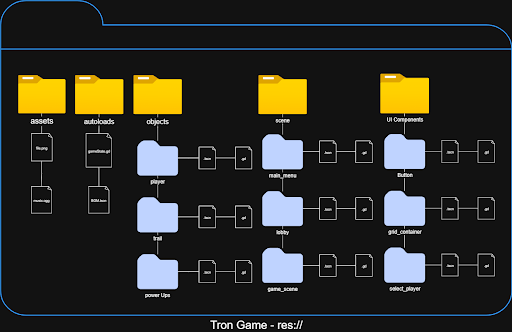
\includegraphics[width=0.7\textwidth]{figuras/diagrama-arquivos.png}
    \legend{Fonte: Elaboração própria}
\end{figure}

\subsection{Interface e usabilidade}

No projeto, a interface e a usabilidade foram estruturadas em três telas principais: o menu inicial, a seleção de jogadores (lobby) e a \texttt{GameScene}. A engine Godot oferece um sistema de construção de interfaces com baixa dependência de código (\textit{low-code}), permitindo o ajuste de tamanhos, textos e posicionamento de \texttt{Containers} diretamente no editor 2D. A integração desses nós a scripts possibilita a conexão de sinais e a atribuição de métodos aos componentes interativos, proporcionando controle total sobre o comportamento da interface.

\begin{figure}[htbp]
    \centering
    \caption{Conexão de nós com scripts no editor Godot.}
    \label{fig:conexao-nos}
    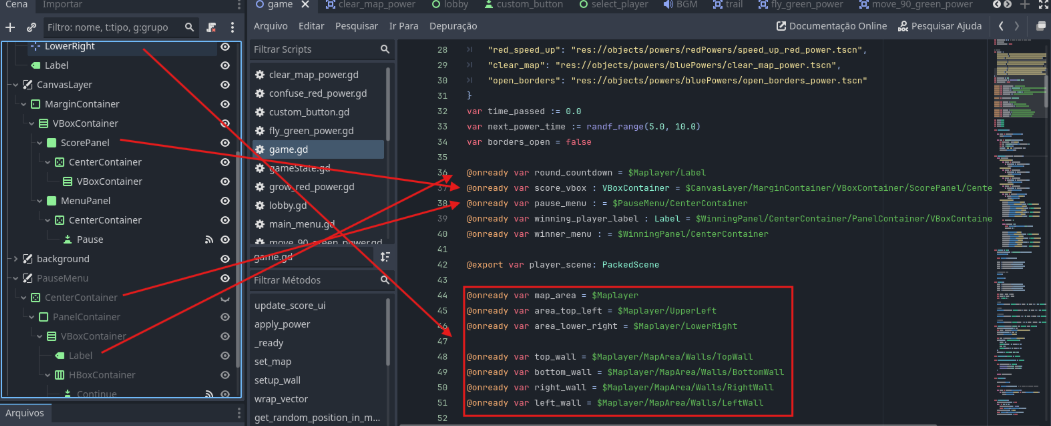
\includegraphics[width=0.7\textwidth]{figuras/conexoes-nos.png}
    \legend{Fonte: Elaboração própria}
\end{figure}

Nas telas de menu, foram utilizados exclusivamente nós do tipo \texttt{Control}, explorando recursos como \textit{Anchors} e \textit{Size Flags} para garantir o alinhamento e o dimensionamento automáticos de painéis, labels e botões em diferentes resoluções. Na \texttt{GameScene}, a raiz da cena é um \texttt{Node2D}, o que facilita a renderização e o posicionamento de elementos gráficos em 2D, mantendo a interface separada em camadas por meio do uso de \texttt{CanvasLayer}, evitando interferência entre a lógica da interface e a lógica de jogo.

Com o objetivo de aprimorar a experiência do usuário, duas funcionalidades específicas foram implementadas. A primeira consiste na personalização dos comandos de movimento (\textit{keybinds}) no lobby, com armazenamento das configurações no singleton \texttt{GameManager}, permitindo a persistência das escolhas entre as rodadas. A segunda funcionalidade é a exibição de uma seta direcional sobre o veículo de cada jogador no início de cada rodada, indicando sua orientação inicial e contribuindo para uma melhor percepção espacial logo nos primeiros movimentos. Tais melhorias foram planejadas para oferecer maior clareza visual e controle aos participantes durante a partida.

Além disso, sons foram adicionados para reforçar a imersão do jogador e dar feedbacks importantes durante o jogo. A música de fundo é gerenciada por meio de um \texttt{AudioStreamPlayer} inserido em um nó global no \textit{AutoLoad}, configurado para reprodução contínua em loop entre as cenas. Já os efeitos sonoros específicos, como o som de morte do jogador, foram implementados diretamente em suas respectivas cenas (Player.tscn). Para isso, utilizou-se o nó \texttt{AudioStreamPlayer2D}, permitindo que cada jogador reproduza sons de forma independente e com espacialização adequada, sem comprometer a lógica principal do jogo.

\subsection{Implementação das mecânicas do jogo}

O desenvolvimento foi feito em GDScript, a linguagem nativa da Godot. Ela é baseada em Python e é fortemente integrada à arquitetura da engine. Três métodos se destacam na construção da lógica do jogo: \texttt{ready}, chamado uma vez assim que o nó entra na árvore de cena; \texttt{physics\_process(delta)}, executado a cada frame de física e utilizado para atualizar elementos em tempo real; e a anotação \texttt{@onready}, que permite inicializar variáveis com nós da cena somente após estarem carregados. Esses recursos estruturam o ciclo de vida dos objetos e organizam a execução do jogo em etapas previsíveis. Além disso, a engine Godot adota uma estrutura orientada a nós, onde tudo é tratado como um objeto independente na hierarquia da cena. Qualquer referência a esse objeto, quando alterada, reflete automaticamente em todas as partes do código onde ele está instanciado ou referenciado, o que facilita a reutilização, modularização e manutenção do projeto.

O \texttt{ready} carrega a cena inicial. Define as dimensões do mapa e chamado a função de \texttt{start\_round} que dá início ao jogo.

A função \texttt{start\_round} é chamada no início de cada rodada e tem como responsabilidade configurar o estado inicial do jogo. Nela são instanciados os jogadores, com base em uma cena pré-configurada (\texttt{PackedScene}), posicionados nos marcadores definidos no mapa e conectados aos seus respectivos sinais. Além disso, o método define o tempo para início da rodada, ativando um contador regressivo e liberando o movimento dos jogadores apenas após sua conclusão. Esse controle inicial garante que todas as partidas comecem de forma sincronizada e clara para os participantes.

\begin{figure}[htbp]
    \centering
    \caption{código: round\_start}
    \label{fig:round_start}
    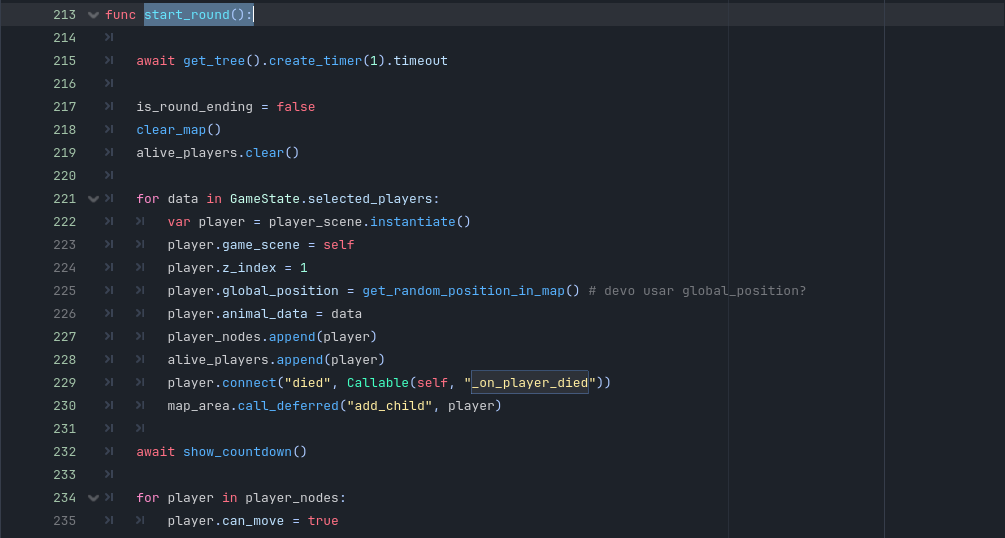
\includegraphics[width=0.7\textwidth]{figuras/round_start.png}
    \legend{Fonte: Elaboração própria}
\end{figure}

Durante a execução do jogo, a função \texttt{physics\_process(delta)} é responsável por atualizar o tempo, movimentar os jogadores e controlar os poderes. Cada jogador move-se em linha reta com velocidade constante, ajustando sua rotação com base nas entradas recebidas. A cada ciclo de atualização, o jogo verifica se é hora de instanciar um novo rastro atrás do jogador, formando a trilha que delimita o espaço percorrido. Também é nesse método que o cronômetro de geração de poderes é verificado, e, ao atingir o tempo definido, um novo poder é instanciado em posição aleatória no mapa.

\begin{figure}[htbp]
    \centering
    \caption{gamescene: \_physics\_process}
    \label{fig:player_pp}
    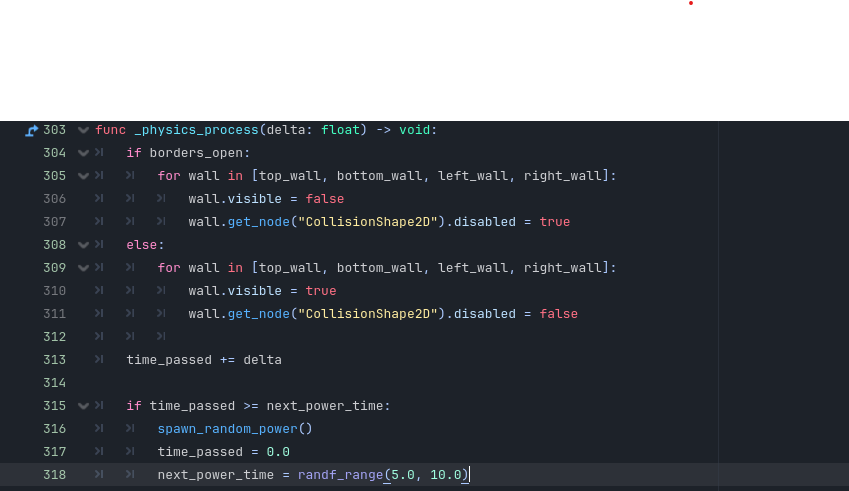
\includegraphics[width=0.7\textwidth]{figuras/game_process.png}
    \legend{Fonte: Elaboração própria}
\end{figure}

\begin{figure}[htbp]
    \centering
    \caption{player: \_physics\_process}
    \label{fig:gamascene_pp}
    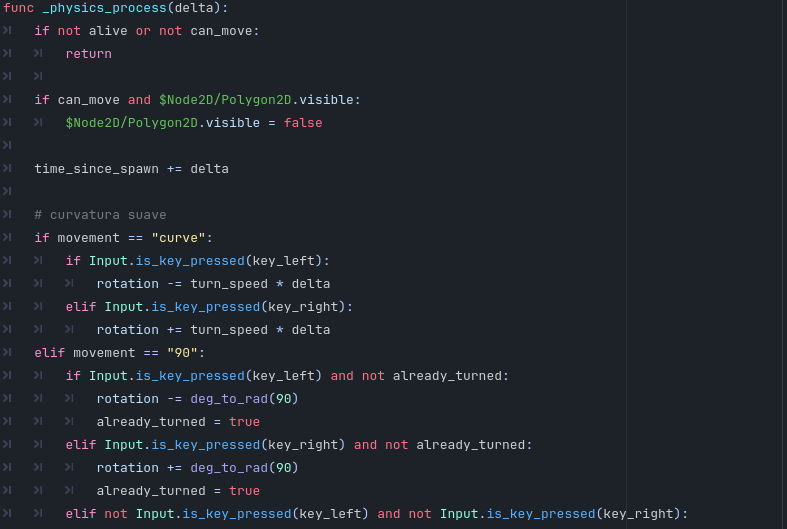
\includegraphics[width=0.7\textwidth]{figuras/player_process.png}
    \legend{Fonte: Elaboração própria}
\end{figure}

A detecção de colisões foi feita por meio do nó \texttt{Area2D} com \texttt{CollisionShape2D}, presente tanto nos jogadores quanto nos rastros e paredes. Cada jogador possui um sinal \texttt{area\_entered} conectado diretamente à cena \texttt{GameScene}, utilizando \texttt{Callable(self, "\_on\_player\_died")}. Ao detectar uma colisão com uma área pertencente a outro jogador, a função de morte é acionada, removendo o jogador da cena e atualizando o ranking da rodada. A função \texttt{end\_round}, chamada após restar apenas um jogador vivo, é responsável por pausar o jogo, distribuir os pontos com base na ordem de eliminação, verificar se algum jogador alcançou a pontuação de vitória e, caso não haja vencedor, iniciar uma nova rodada com \texttt{start\_round}.

\begin{figure}[htbp]
    \centering
    \caption{gamescene: \_on\_player\_died}
    \label{fig:on_player_died}
    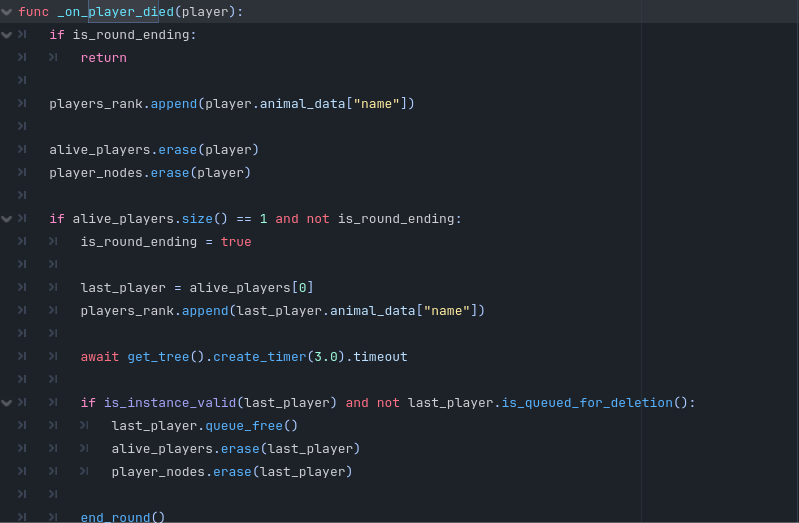
\includegraphics[width=0.7\textwidth]{figuras/game_body.png}
    \legend{Fonte: Elaboração própria}
\end{figure}

\begin{figure}[htbp]
    \centering
    \caption{player: \_on\_area\_entered}
    \label{fig:player_area_func}
    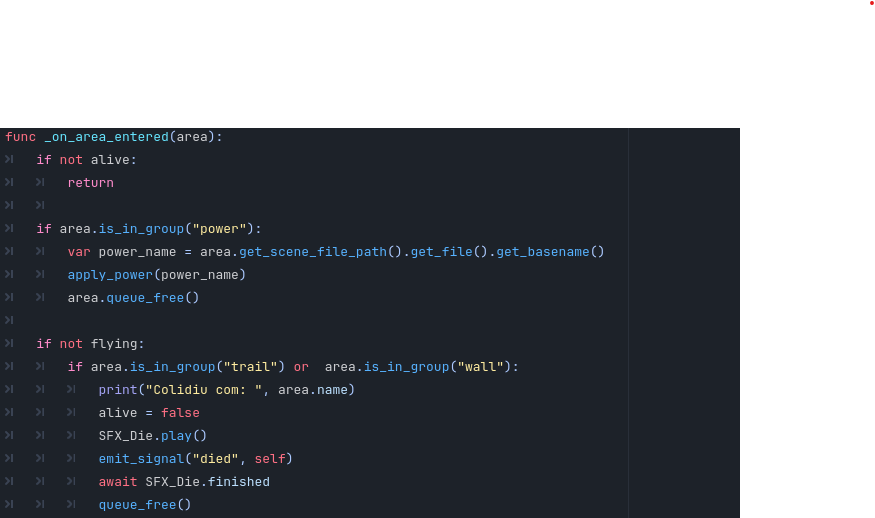
\includegraphics[width=0.7\textwidth]{figuras/player_body.png}
    \legend{Fonte: Elaboração própria}
\end{figure}

Para o áudio, foi adotada uma abordagem simples e funcional. A música de fundo é gerenciada por um nó \texttt{AudioStreamPlayer}, carregado por meio de um script no \texttt{AutoLoad}, o que permite sua reprodução contínua em loop durante todo o jogo, independentemente da cena ativa. Já os efeitos sonoros, como o som de morte, foram incorporados diretamente à cena de cada jogador, utilizando o nó \texttt{AudioStreamPlayer2D}. Essa escolha permite que cada instância de jogador reproduza seus próprios sons de forma independente, garantindo uma espacialização adequada e mantendo o controle de áudio encapsulado no próprio objeto responsável pela ação.

Abaixo tem o a fluxo lógico simplificado que ocorre na cena de jogo.

\begin{figure}[htbp]
    \centering
    \caption{BPMN: fluxo lógico}
    \label{fig:bpmn}
    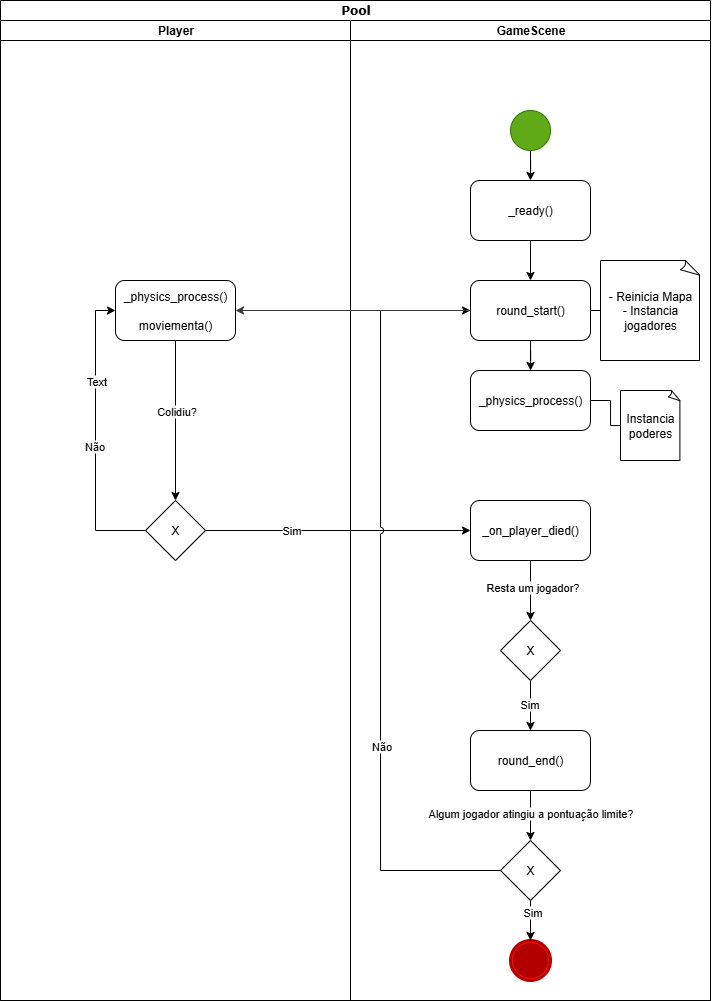
\includegraphics[width=0.7\textwidth]{figuras/BPMN_tcc.png}
    \legend{Fonte: Elaboração própria}
\end{figure}

\begin{table}[H]
\centering
\caption{Tabela de solução de implementação das funcionalidades}
\label{tab:implementacao-funcionalidades}
\begin{tabular}{|p{3.5cm}|p{4cm}|p{7cm}|}
\hline
\textbf{Funcionalidade} & \textbf{Principais nós} & \textbf{Descrição resumida da implementação} \\
\hline
Movimentação & Player (Area2D), Polygon2D, CollisionShape2D e AudioStreamPlayer2D & Usa \texttt{Input.is\_key\_pressed} para ajustar a direção dentro do \texttt{physics\_process} e possui velocidade variável que determina curvas mais fechadas ou abertas. \\
\hline
Rastros & Trail (Node2D), Polygon2D, CollisionShape2D & A cada frame um ponto é adicionado no mapa com a mesma proporção do Player. Esses pontos, em sequência, criam uma linha. \\
\hline
Poderes Especiais & PowerUp (Node2D), Sprite2D, CollisionShape2D & Quando o jogador colide com um PowerUp, altera atributos do jogador (ex.: velocidade, invulnerabilidade) ou das paredes do mapa dentro do \texttt{GameManager}. \\
\hline
Colisão e eliminação & Embutido nos rastros, jogadores e paredes, signal \texttt{body\_entered} através do CollisionShape2D & Conecta o sinal de eliminação ao método que verifica se o jogador tocou parede ou rastro alheio; em caso positivo, notifica o \texttt{GameManager} e o próprio objeto remove sua instância do jogo. \\
\hline
Sistema de pontos & Singleton \texttt{GameManager}, Label de HUD & Mantém dicionário de pontuações; ao final de cada rodada calcula ordem de eliminação, atualiza as \texttt{labels} e declara fim da partida. \\
\hline
Tamanho do mapa & Dois \texttt{Marker2D} e quatro \texttt{Walls} (Area2D) & Os marcadores delimitam as bordas do mapa e as paredes, com as coordenadas dos marcadores, são instanciadas na cena. \\
\hline
\end{tabular}

\vspace{0.3em}
\small \textbf{Fonte:} Elaboração própria.
\end{table}

\subsection{Fluxo de telas e linha de desenvolvimento}

O fluxo de telas do jogo consiste em três cenas: menu principal, lobby e jogo. Abaixo é possível visualizar o resultado final e a sequência de tela do jogo.

A tela inicial possui um \textit{background} com estética semelhante ao jogo, e o usuário pode optar por sair do jogo ou jogar através de um clique.

\begin{figure}[htbp]
    \centering
    \caption{Tela menu inicial.}
    \label{fig:menu-inical}
    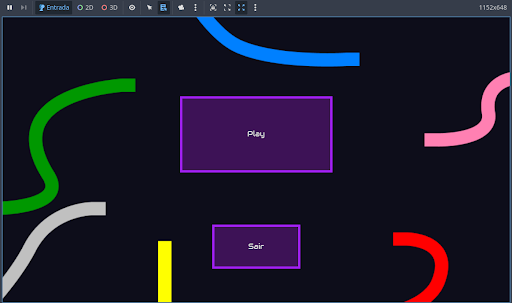
\includegraphics[width=0.7\textwidth]{figuras/menu-game.png}
    \legend{Fonte: Elaboração própria}
\end{figure}

Na tela de Lobby tem a opção de jogar com até 6 jogadores e cada jogador pode customizar suas teclas de comando. É possível remover um jogadores caso necessário e continuar para o jogo.

\begin{figure}[htbp]
    \centering
    \caption{Tela do Lobby do jogo.}
    \label{fig:menu-lobby}
    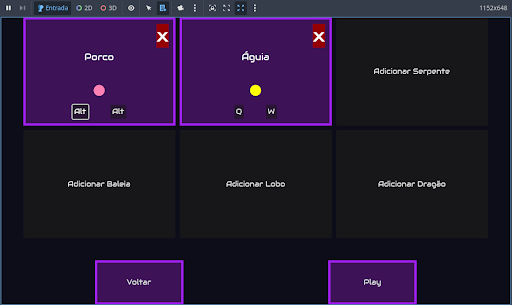
\includegraphics[width=0.7\textwidth]{figuras/lobby-game.png}
    \legend{Fonte: Elaboração própria}
\end{figure}

Na cena do jogo, temos um painel com a pontuação dos jogadores, um botão de pause, um contador que declara início da rodada e três jogadores dispostos no mapa com indicadores de suas atuais direções.

\begin{figure}[htbp]
    \centering
    \caption{Tela do jogo com indicadores de direção antes de começar a rodada.}
    \label{fig:in-game}
    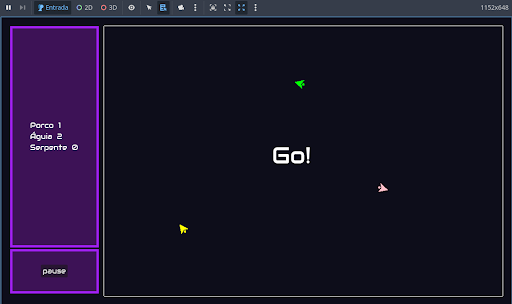
\includegraphics[width=0.7\textwidth]{figuras/in-game.png}
    \legend{Fonte: Elaboração própria}
\end{figure}

O jogo pode ser pausado a qualquer momento oferecendo as opções de voltar ou continuar a partida.

\begin{figure}[htbp]
    \centering
    \caption{Tela do jogo em pause.}
    \label{fig:pause-game}
    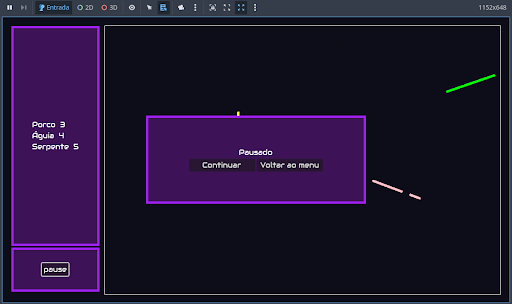
\includegraphics[width=0.7\textwidth]{figuras/pause-menu.png}
    \legend{Fonte: Elaboração própria.}
\end{figure}

Quando um jogador alcança a pontuação mínima, o jogo encerra declarando o vencedor seguido de um botão de continuar.

\begin{figure}[htbp]
    \centering
    \caption{Tela do jogo encerrado.}
    \label{fig:fim-do-game}
    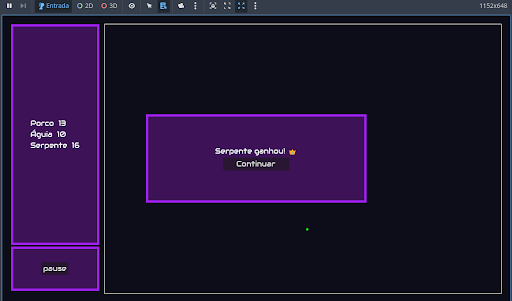
\includegraphics[width=0.7\textwidth]{figuras/win-game.png}
    \legend{Fonte: Elaboração própria.}
\end{figure}

\subsection{Principais desafios e soluções}

Durante o desenvolvimento do jogo, diversos desafios técnicos e conceituais surgiram, especialmente por se tratar da primeira experiência prática com uma engine de jogos. O primeiro obstáculo foi compreender o funcionamento da Godot Engine e explorar suas funcionalidades. Para isso, foi essencial adotar uma abordagem de aprendizagem baseada em experimentação contínua, consulta à documentação oficial, fóruns, vídeos e o uso de inteligência artificial para suporte na resolução de problemas. A própria engine facilita esse processo ao oferecer uma documentação embutida que permite explorar métodos e propriedades diretamente nos nós utilizados.

Um segundo desafio relevante foi a construção da interface. A tentativa de criar telas responsivas exigiu o entendimento aprofundado sobre propriedades como ancoragem, margens, alinhamentos e retângulos (\texttt{Rect}). Além disso, foi necessário aprender a combinar diferentes tipos de \texttt{Container} para estruturar layouts adaptáveis, utilizando ferramentas como \texttt{HBoxContainer}, \texttt{VBoxContainer} e \texttt{MarginContainer}.

A elaboração da lógica principal do jogo representou outro desafio. Por ser baseada em uma estrutura de nós hierárquicos, o desenvolvedor precisa entender a relação entre os elementos, como a importância de posicionar corretamente objetos filhos em relação ao pai, além de saber gerenciar sua comunicação por meio de sinais e grupos. No início, quando ainda não há uma versão testável do jogo, muitos conceitos permanecem meio que abstratos, por isso é comum implementar diversas funcionalidades sem conseguir visualizar seu comportamento final. Isso exige um processo constante de revisão e adaptação, à medida que o restante da estrutura vai sendo integrada e testada.

Entre os problemas práticos mais complexos esteve a criação do rastro deixado pelos jogadores em movimento, principal elemento do jogo. A primeira abordagem testada foi o uso de um \texttt{Line2D}, que conectava os pontos por onde o jogador passava. Inicialmente era funcional. Porém, essa solução apresentou falhas ao lidar com teletransporte. Ao atravessar a borda do mapa, um traço era desenhado ligando pontos opostos da tela. A solução adotada foi instanciar, em intervalos curtos, múltiplos rastros independentes com aparência igual à do jogador, que juntos formam uma linha visualmente contínua.

Outro problema significativo ainda relacionado ao rastro foi a colisão imediata do jogador com o próprio traço recém-gerado, o que tornava a partida impossível de continuar. Três alternativas foram testadas: aplicar um pequeno atraso antes de instanciar o rastro, adicionar uma distância mínima entre o jogador e o ponto de criação do rastro, e finalmente, a abordagem escolhida: aguardar que o jogador deixe a área de colisão do rastro antes de adicioná-lo ao grupo responsável por registrar colisões (grupo \texttt{"trail"}). Essa última estratégia demonstrou-se mais confiável e garantiu a jogabilidade esperada, mas ainda com problemas.

Após a implementação de todos os poderes, aqueles que alteravam o tamanho dos jogadores ainda apresentavam comportamentos inconsistentes, sem uma solução satisfatória no momento. Diante disso, optou-se por remover temporariamente esses poderes do jogo, até que uma abordagem mais estável e compatível com o restante da lógica fosse encontrada.

Ao longo do desenvolvimento, diversos outros problemas surgiram, de escala menor ou semelhante, mas ainda assim relevantes para o processo de aprendizagem. Alguns foram resolvidos rapidamente, enquanto outros exigiram maior abstração e análise do comportamento da engine. Entre os exemplos recorrentes estavam situações como instanciar objetos como filhos de outros e perceber que isso altera sua \texttt{global\_position}, ou tentar interagir com nós que já haviam sido removidos. Com o tempo, esses padrões de erro se tornam mais reconhecíveis, e a experiência adquirida passa a desempenhar um papel fundamental na antecipação de problemas e na escolha de soluções mais eficientes. Esses aprendizados acumulados, ainda que muitas vezes não documentados diretamente, contribuem significativamente para a formação prática do desenvolvedor.

\subsection{Testes de Funcionalidade e Desempenho}

Os testes realizados no projeto seguiram uma abordagem prática e limitada, considerando os recursos disponíveis. A metodologia adotada foi a de testes manual de caixa-preta, com foco na verificação do comportamento esperado das funcionalidades implementadas, sem considerar a estrutura interna do código. Essa abordagem é comum em projetos de software com restrições de tempo ou equipe reduzida, como é o caso deste trabalho \cite{pinheiro2024testes} \cite{checkpoint_blackbox}.

Os testes foram realizados pelo próprio autor, de forma exploratória, em um ambiente local, utilizando um computador pessoal com sistema Windows 11, AMD Ryzen 5 3600 6-Core Processor, 16 GB memória RAM, placa de vídeo AMD Radeon RX 5600 XT.

Durante o processo de testes, foram identificados bugs e comportamentos inesperados, como colisões incorretas, travamentos de movimentos ou falhas em efeitos visuais. Esses problemas eram registrados na plataforma Trello, dentro da seção de tarefas “Melhorias”, para posterior análise e correção. Esse processo, ainda que informal, foi essencial para garantir a estabilidade mínima do sistema e evitar que erros simples passassem despercebidos até a entrega final.

\begin{figure}[htbp]
    \centering
    \caption{Quadro - Polimento e Ajustes}
    \label{fig:polimento-e-ajustes}
    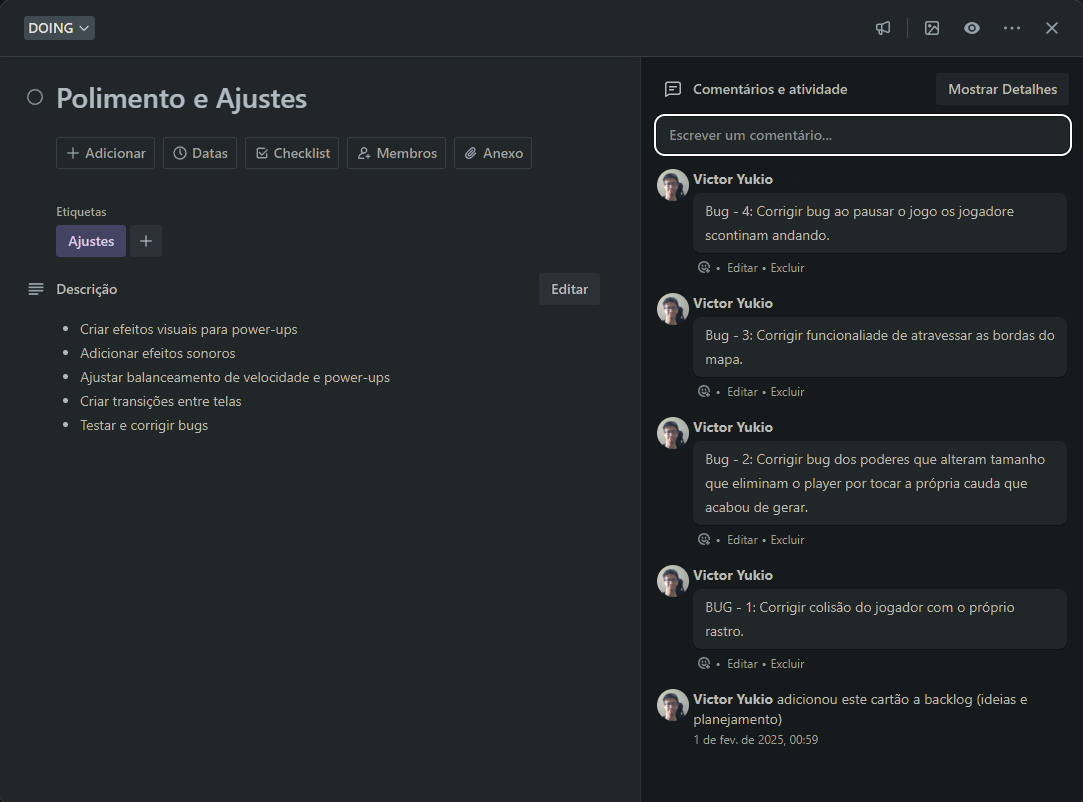
\includegraphics[width=0.7\textwidth]{figuras/bugs-tcc.png}
    \legend{Fonte: Elaboração própria}
\end{figure}

Além da detecção de falhas, os testes também desempenharam um papel fundamental no balanceamento das mecânicas do jogo. Durante as sessões de teste, foi possível observar, por exemplo, se a velocidade base dos jogadores proporcionava uma movimentação justa, se o tempo de duração dos poderes estava adequado para não desestabilizar as partidas e se os controles respondiam de forma fluida. Pequenas observações sobre o  comportamento em jogo que contribuindo para a melhoria da experiência geral e diversão dos jogadores.

Apesar das limitações, o processo de testes contribuiu para a melhoria contínua do jogo, permitindo a identificação e correção de falhas ao longo do desenvolvimento. A prática de documentar os problemas e tratá-los como parte do ciclo de produção reforçou o valor da organização e da iteração constante no desenvolvimento de software.
